\chapter{Results}\label{ch:results}

In this chapter we evaluate the path prediction system: first we describe how our system can emulate OSPF by analyzing the results of the model training; finally we discuss the performance of the path prediction model as a substitute to the traditional routing algorithms.

\section{Learning from OSPF}
The system is built to learn OSPF behavior in different configurations and correlate it with the traffic patterns. We use a LSTM RNN as a learning algorithm and build a model for each source-destination pair in our topology (figure~\ref{fig:topology}): the total number of models is given by the all the possible $(src\_router, dst\_addr)$ pairs, with the destination addresses considered only on the outer routers different from the source; given a router, the number of addresses associated to it, is equal to the number of its interfaces. The result is a set of $162$ models which are used to determine the hop-by-hop path from a source router to a specific destination address. The whole path is computed as follows: starting from the source, the model for the selected destination is used to predict the next hop, then the predicted next hop becomes the new source router and the process is repeated until the predicted hop is the final destination. Given their high number, it is not feasible to analyze all models individually; moreover, we are interested in exploring the overall performance. To do so, we analyze the average accuracy and loss over the different models, as discussed in the previous chapter.

Figure~\ref{fig:training_avg} shows the model training progress over time in terms of accuracy and loss: the plot is the average of the metrics over the $162$ models. The slopes of the graphs give us an idea of what is happening during the training: at the beginning (epochs 0-20), both of the slopes are very steep, indicating that the model is abandoning the initial randomness and moving towards the solution. Afterwards, from epoch 20 to 60, as the gradient diminishes, the slope starts to decrease slowly, indicating that the gradient has probably entered the region of the space in which it will converge to the problem solution. Finally, the curve becomes almost flat, showing that the gradient has reached the problem minimum and cannot improve anymore.It is very important to notice how in both the graphs, the two curves have the same tendency: this is crucial because it shows that the model is learning without losing generality. An increasing accuracy on the training set with a steady or decaying validation accuracy would be a clear sign of overfitting, a situation in which the model becomes too specialized on the training data and it is not able to properly classify new samples.

\begin{figure}
\makebox[\textwidth]{\centering
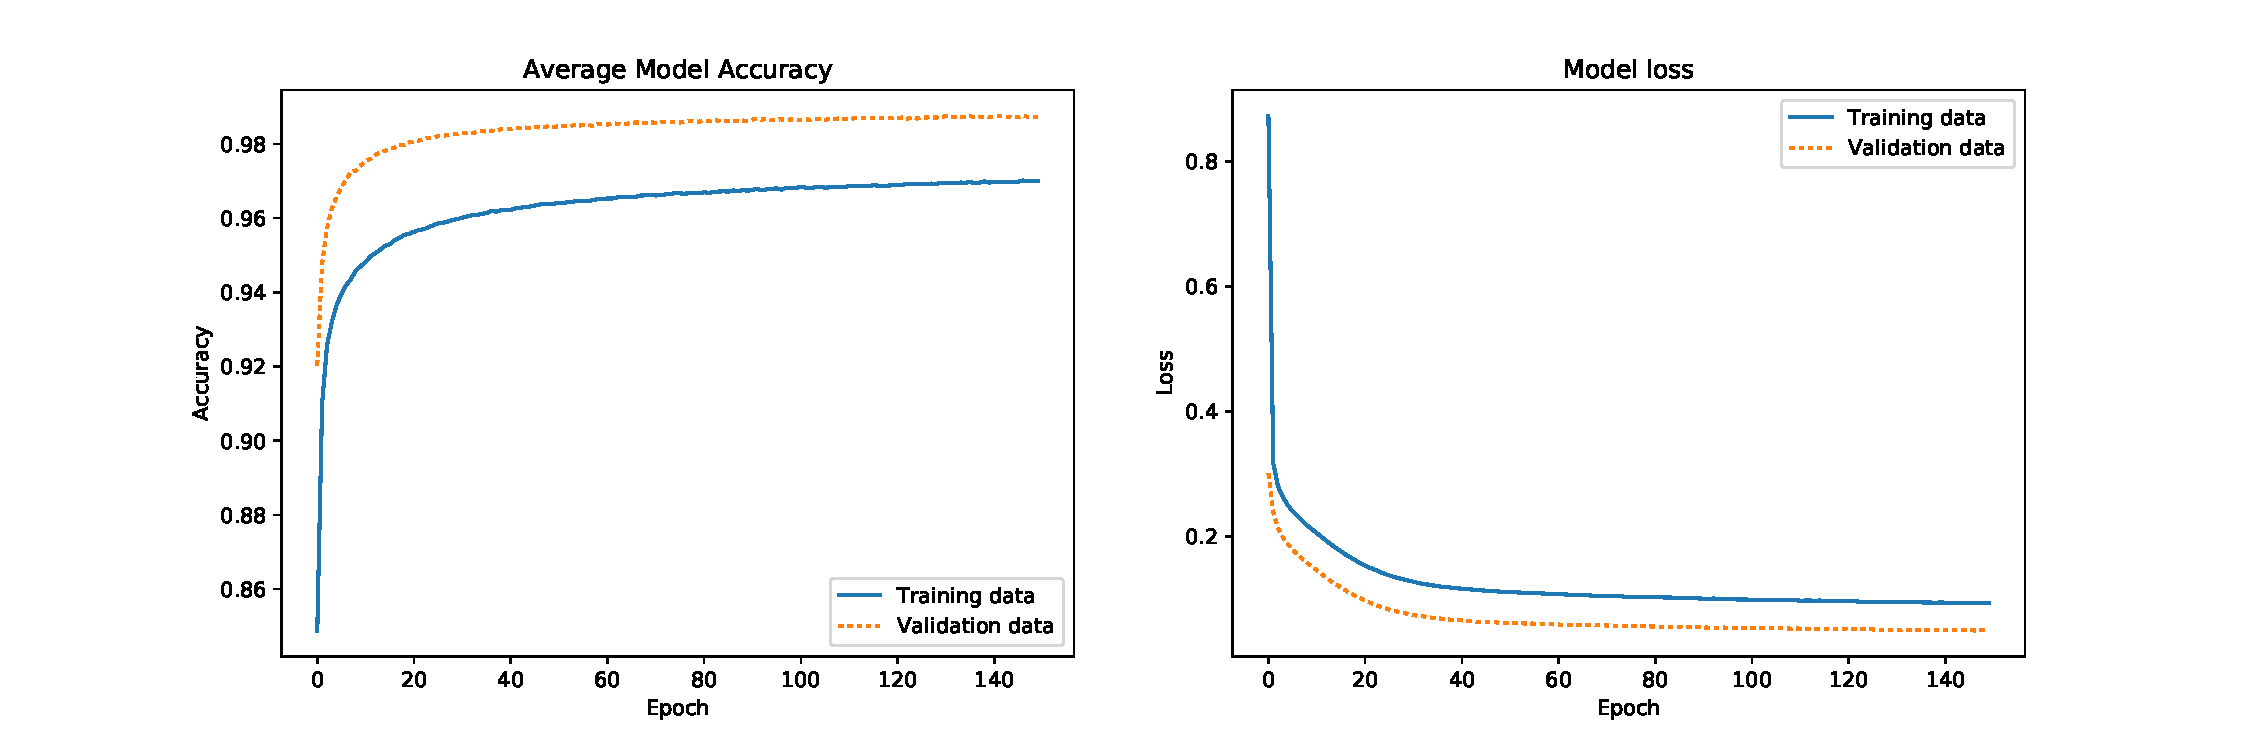
\includegraphics[width=0.88\paperwidth]{img/avg_training_metrics}}
\caption{Training accuracy and loss progress.}
\label{fig:training_avg}
\end{figure}

To understand how well our model can emulate OSPF we need to analyze the performance on the test set; as we did for the training, we evaluate the performance of the system by averaging the results of the single models. The system achieves an average accuracy of $\textbf{98.71\%}$, with a loss of only $\textbf{0.0496}$; showing really promising results. With an accuracy of almost $99\%$, LSTM-RNNs seem to perform better than traditional DNNs~\cite{Kato}; however this comparison should be taken with caution, considered that the topologies in the two experiments are slightly different and experiments reproducibility is an open issue in machine learning~\cite{olorisade2017reproducibility}. It is important to notice that in this case, the average accuracy could be slightly misleading: the models the represents a directly connected target (a source-destination pair connected by a single link), are very simple, so it is very likely for them to have an accuracy close or even equal to $100\%$. Nonetheless, only the $32\%$ (obtained counting all the directly connected target including all the interfaces on the destination router) of the models represents this situation, that means that even if they all had $100\%$ accuracy, the remaining models would have an average accuracy of $97.89\%$.

\section{Replacing OSPF}
To evaluate our model as OSPF replacement, we observe the behavior of the path prediction system in a functioning network. In particular, we  use the same topology (figure~\ref{fig:topology}) and traffic simulator adopted in the dataset generation phase; to ease the analysis process, all the links are set to the same speed. Afterwards, we select a source router and a destination address and examine the difference in behavior between OSPF and our system.

In general, our system shows a dynamic behavior, predicting several paths for the same destination in different traffic conditions. More specifically, we run four traffic simulation, each fifteen minutes long, with a varying loss rate on the link chosen by OSPF to connect source and destination; at the same time, the path prediction system computes a new path every five seconds. The selected target is $(R1, R3)$, with the default path being $R1,R2,R3$ and the loss being varied on the link between R1 and R2. Figure~\ref{fig:path_cmp} compares the routing decisions made by the system in comparisons: being performance unaware, OSPF always chooses the same path, even when the link has losses. Our system on the contrary, shows the ability of behaving dynamically by proposing four alternative paths.

\begin{figure}[h]
\centering
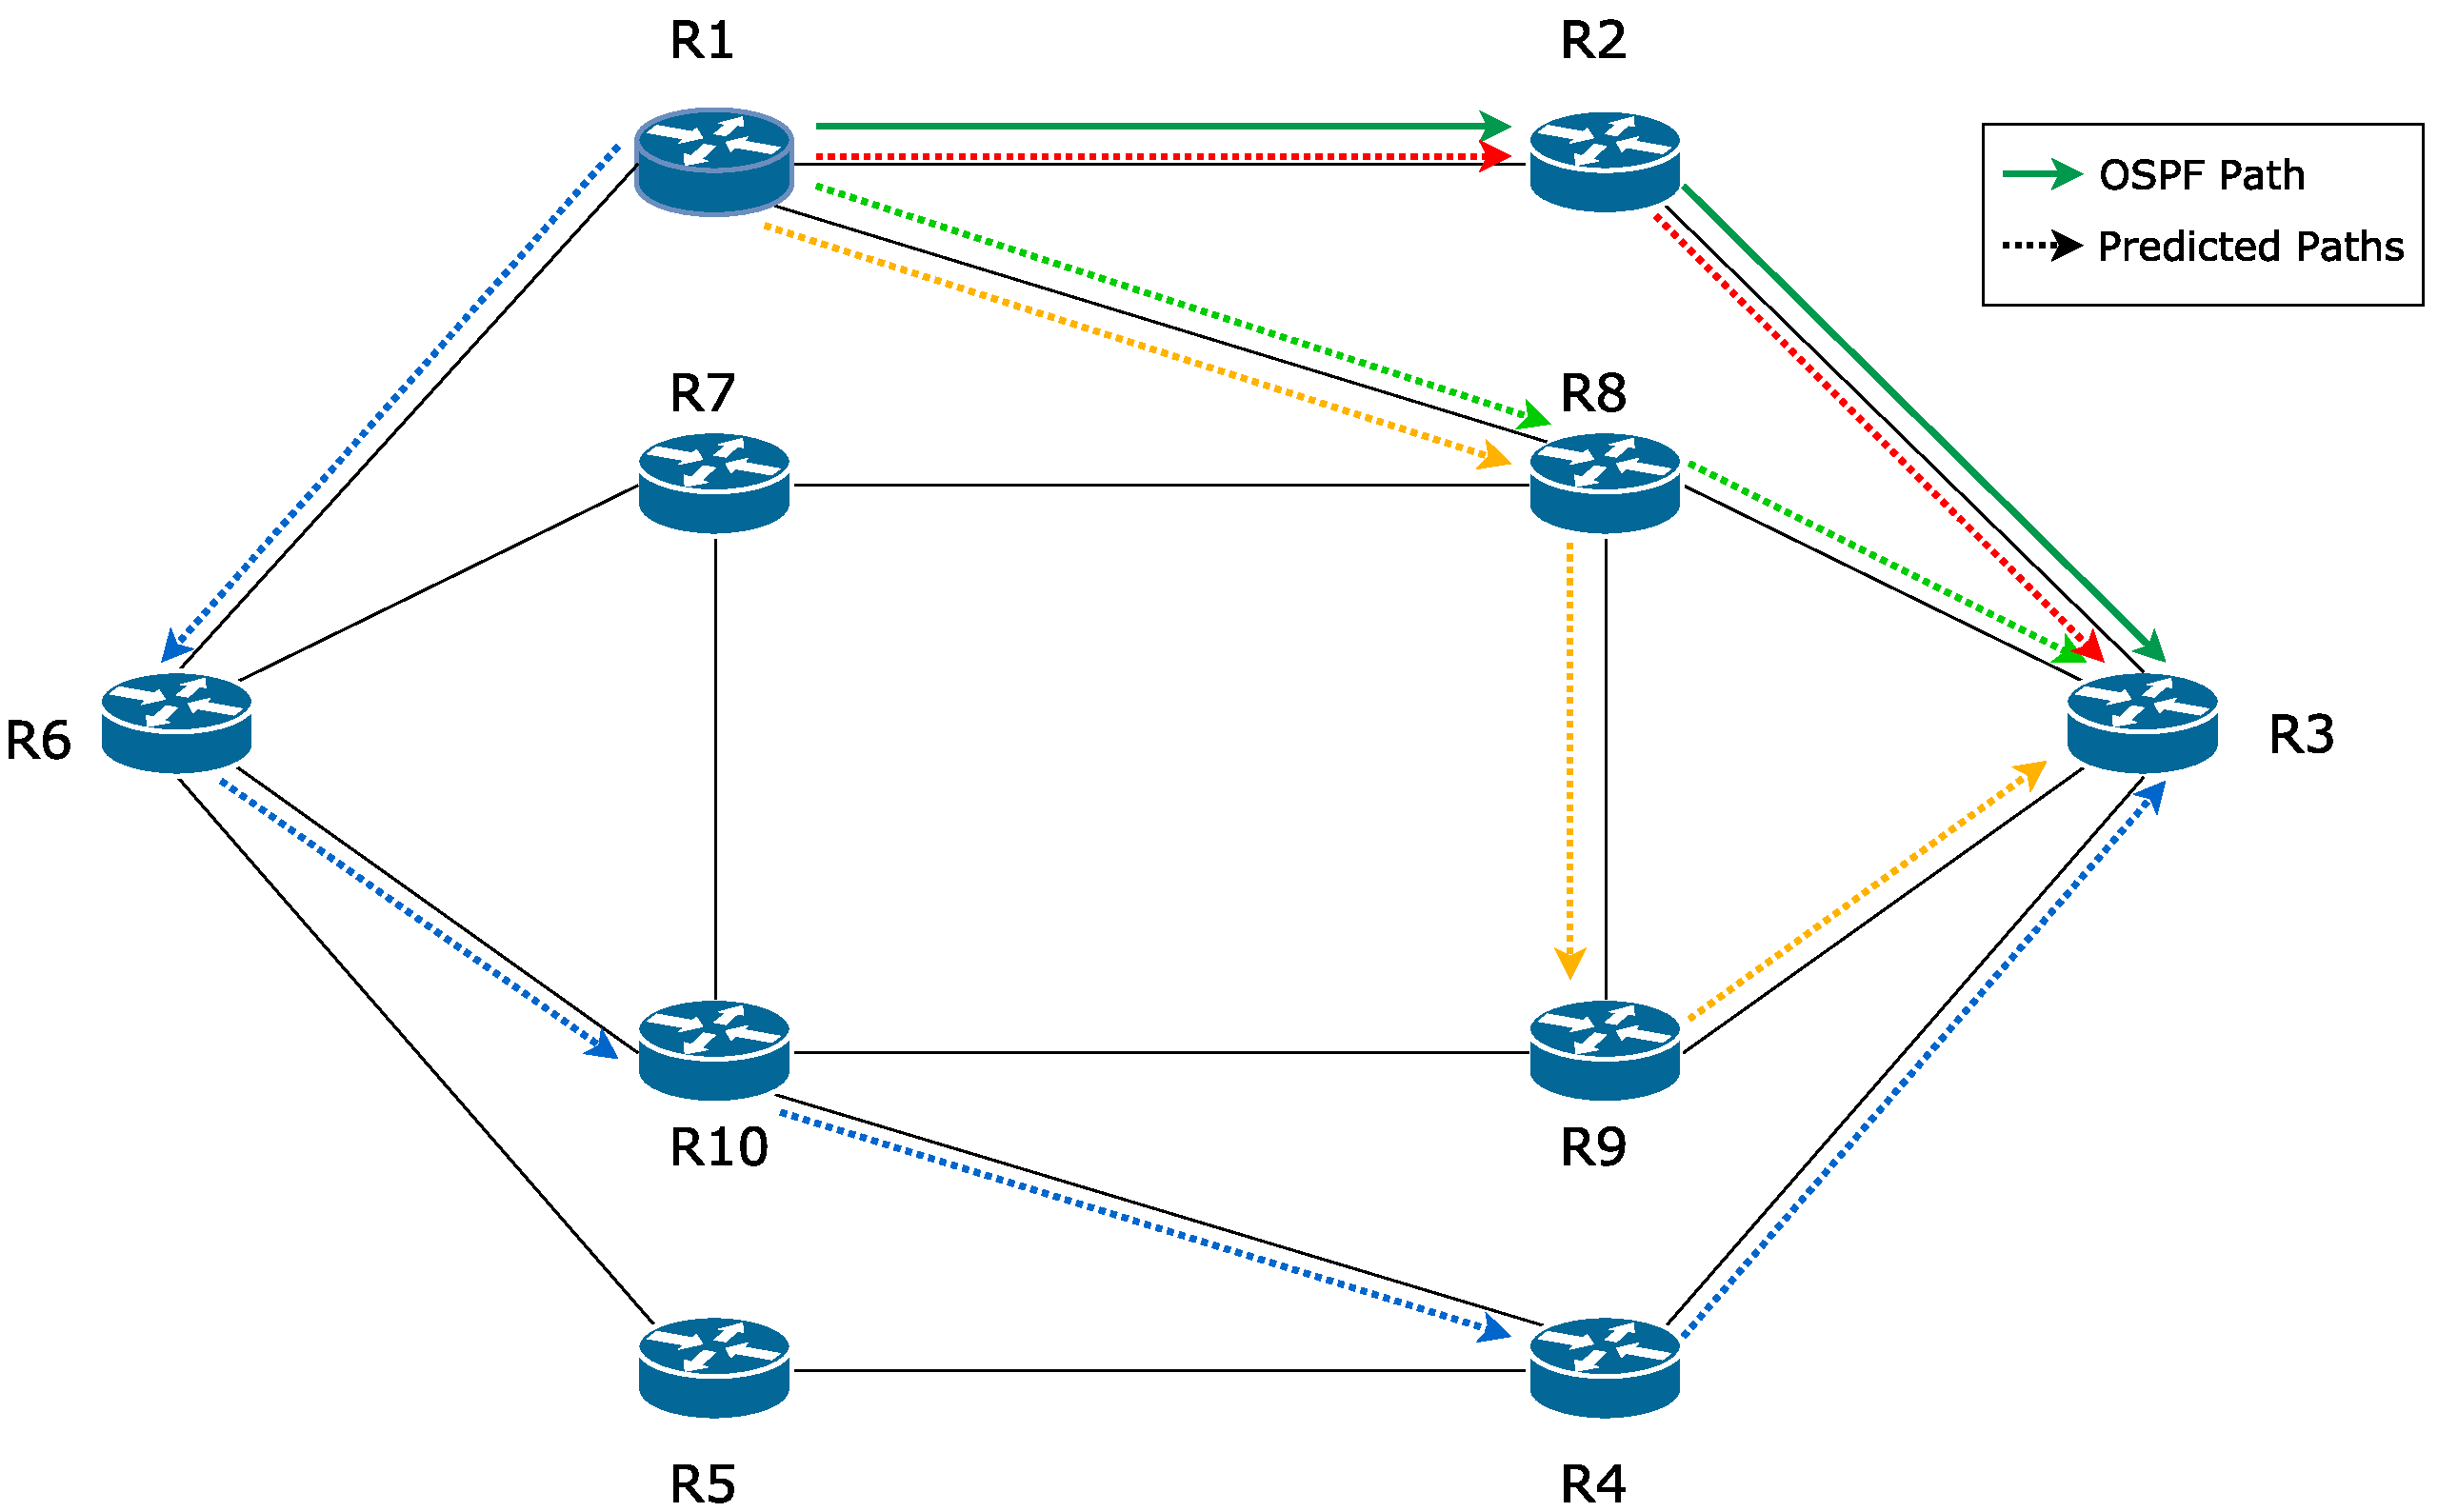
\includegraphics[width=0.82\textwidth]{img/path_comparison}
\caption{Routing policies comparison.}
\label{fig:path_cmp}
\end{figure}
By studying the system behavior in presence of losses, it is possible to understand if our model is able to detect and overcome these problems. We test loss rates of 0\%, 10\%, 15\%, 20\% and count the number of predictions different from OSPF (table~\ref{tab:same_path_rate}). With the loss set to zero, $60.5\%$ of the time the predicted path is different from OSPF; if increased to $10\%$, the ratio of path different from OSPF rises to $63.5\%$, suggesting that the system is able to detect the change. For the successive loss rates, $15\%$ and $20\%$, the performance goes down a little with respectively only a $59.5\%$ and $54.5\%$ different path ratio; the reasons for this loss in performance are discussed in chapter~\ref{ch:conclusion}. The ideal behavior would be for the system to detect the link loss and consequently stop predicting paths going through the damaged link. In our analysis this happens only with a limited loss rate, however, even though not perfect, the results are encouraging.

Table~\ref{tab:retransmission_rate} compares the resulting retransmission rate of our system, OSPF and equal-cost multipath (ECMP) routing strategies. The retransmission rate is computed by taking into account how many times traffic would pass through the leaky link, considering two equal-cost paths for ECMP and the ratios in table~\ref{tab:retransmission_rate} for our system. Overall, the system we propose, has a lower retransmission rate than the other strategies, reaching therefore a higher throughput. Figure~\ref{fig:prediction_cmp} is a graphical comparison of the three strategies, showing the time difference needed to transmit the same amount of data. If there is no loss, the three approaches behave the same, however, as soon as a loss rate is introduced, the gap between the curves increases. This difference becomes bigger as the loss rate increases, however, while it is evident with respect to OSPF, the variation between ECMP and our system is less evident.
\begin{table}[h]
\centering
{%
\begin{tabular}{|c|c|c|}
\hline
\multicolumn{1}{|l|}{\textbf{Link loss}} & \multicolumn{1}{l|}{\textbf{Different path rate}} & \multicolumn{1}{l|}{\textbf{Same OSPF path rate}} \\ \hline
0\% & 60.5\% & 39.5\% \\ \hline
10\% & 63.5\% & 36.5\% \\ \hline
15\% & 59.5\% & 40.5\% \\ \hline
20\% & 54.5\% & 45.5\% \\ \hline
\end{tabular}%
}
\caption{Path predictions different and equal to OSPF}
\label{tab:same_path_rate}
\end{table}


% Please add the following required packages to your document preamble:
% \usepackage{graphicx}

\begin{table}[]
\centering
\resizebox{\textwidth}{!}{%
\begin{tabular}{|c|c|c|c|}
\hline
\multicolumn{1}{|l|}{}  & \multicolumn{3}{c|}{\textbf{Routing Strategy}}                                          \\ \hline
\textbf{Link loss rate} & \textbf{OSPF} & \textbf{Equal-cost multi-path} & \textbf{Path prediction system (LSTM)} \\ \hline
0\%                     & 0\%           & 0\%                            & \textbf{0\%}                           \\ \hline
10\%                    & 10\%          & 5\%                            & \textbf{3.65\%}                        \\ \hline
15\%                    & 15\%          & 7.5\%                          & \textbf{6.07\%}                        \\ \hline
20\%                    & 20\%          & 10\%                           & \textbf{9.1\%}                         \\ \hline
\end{tabular}%
}
\caption{Routing strategies retransmission rate}
\label{tab:retransmission_rate}
\end{table}

\begin{figure}[h!]
\makebox[\textwidth]{\centering
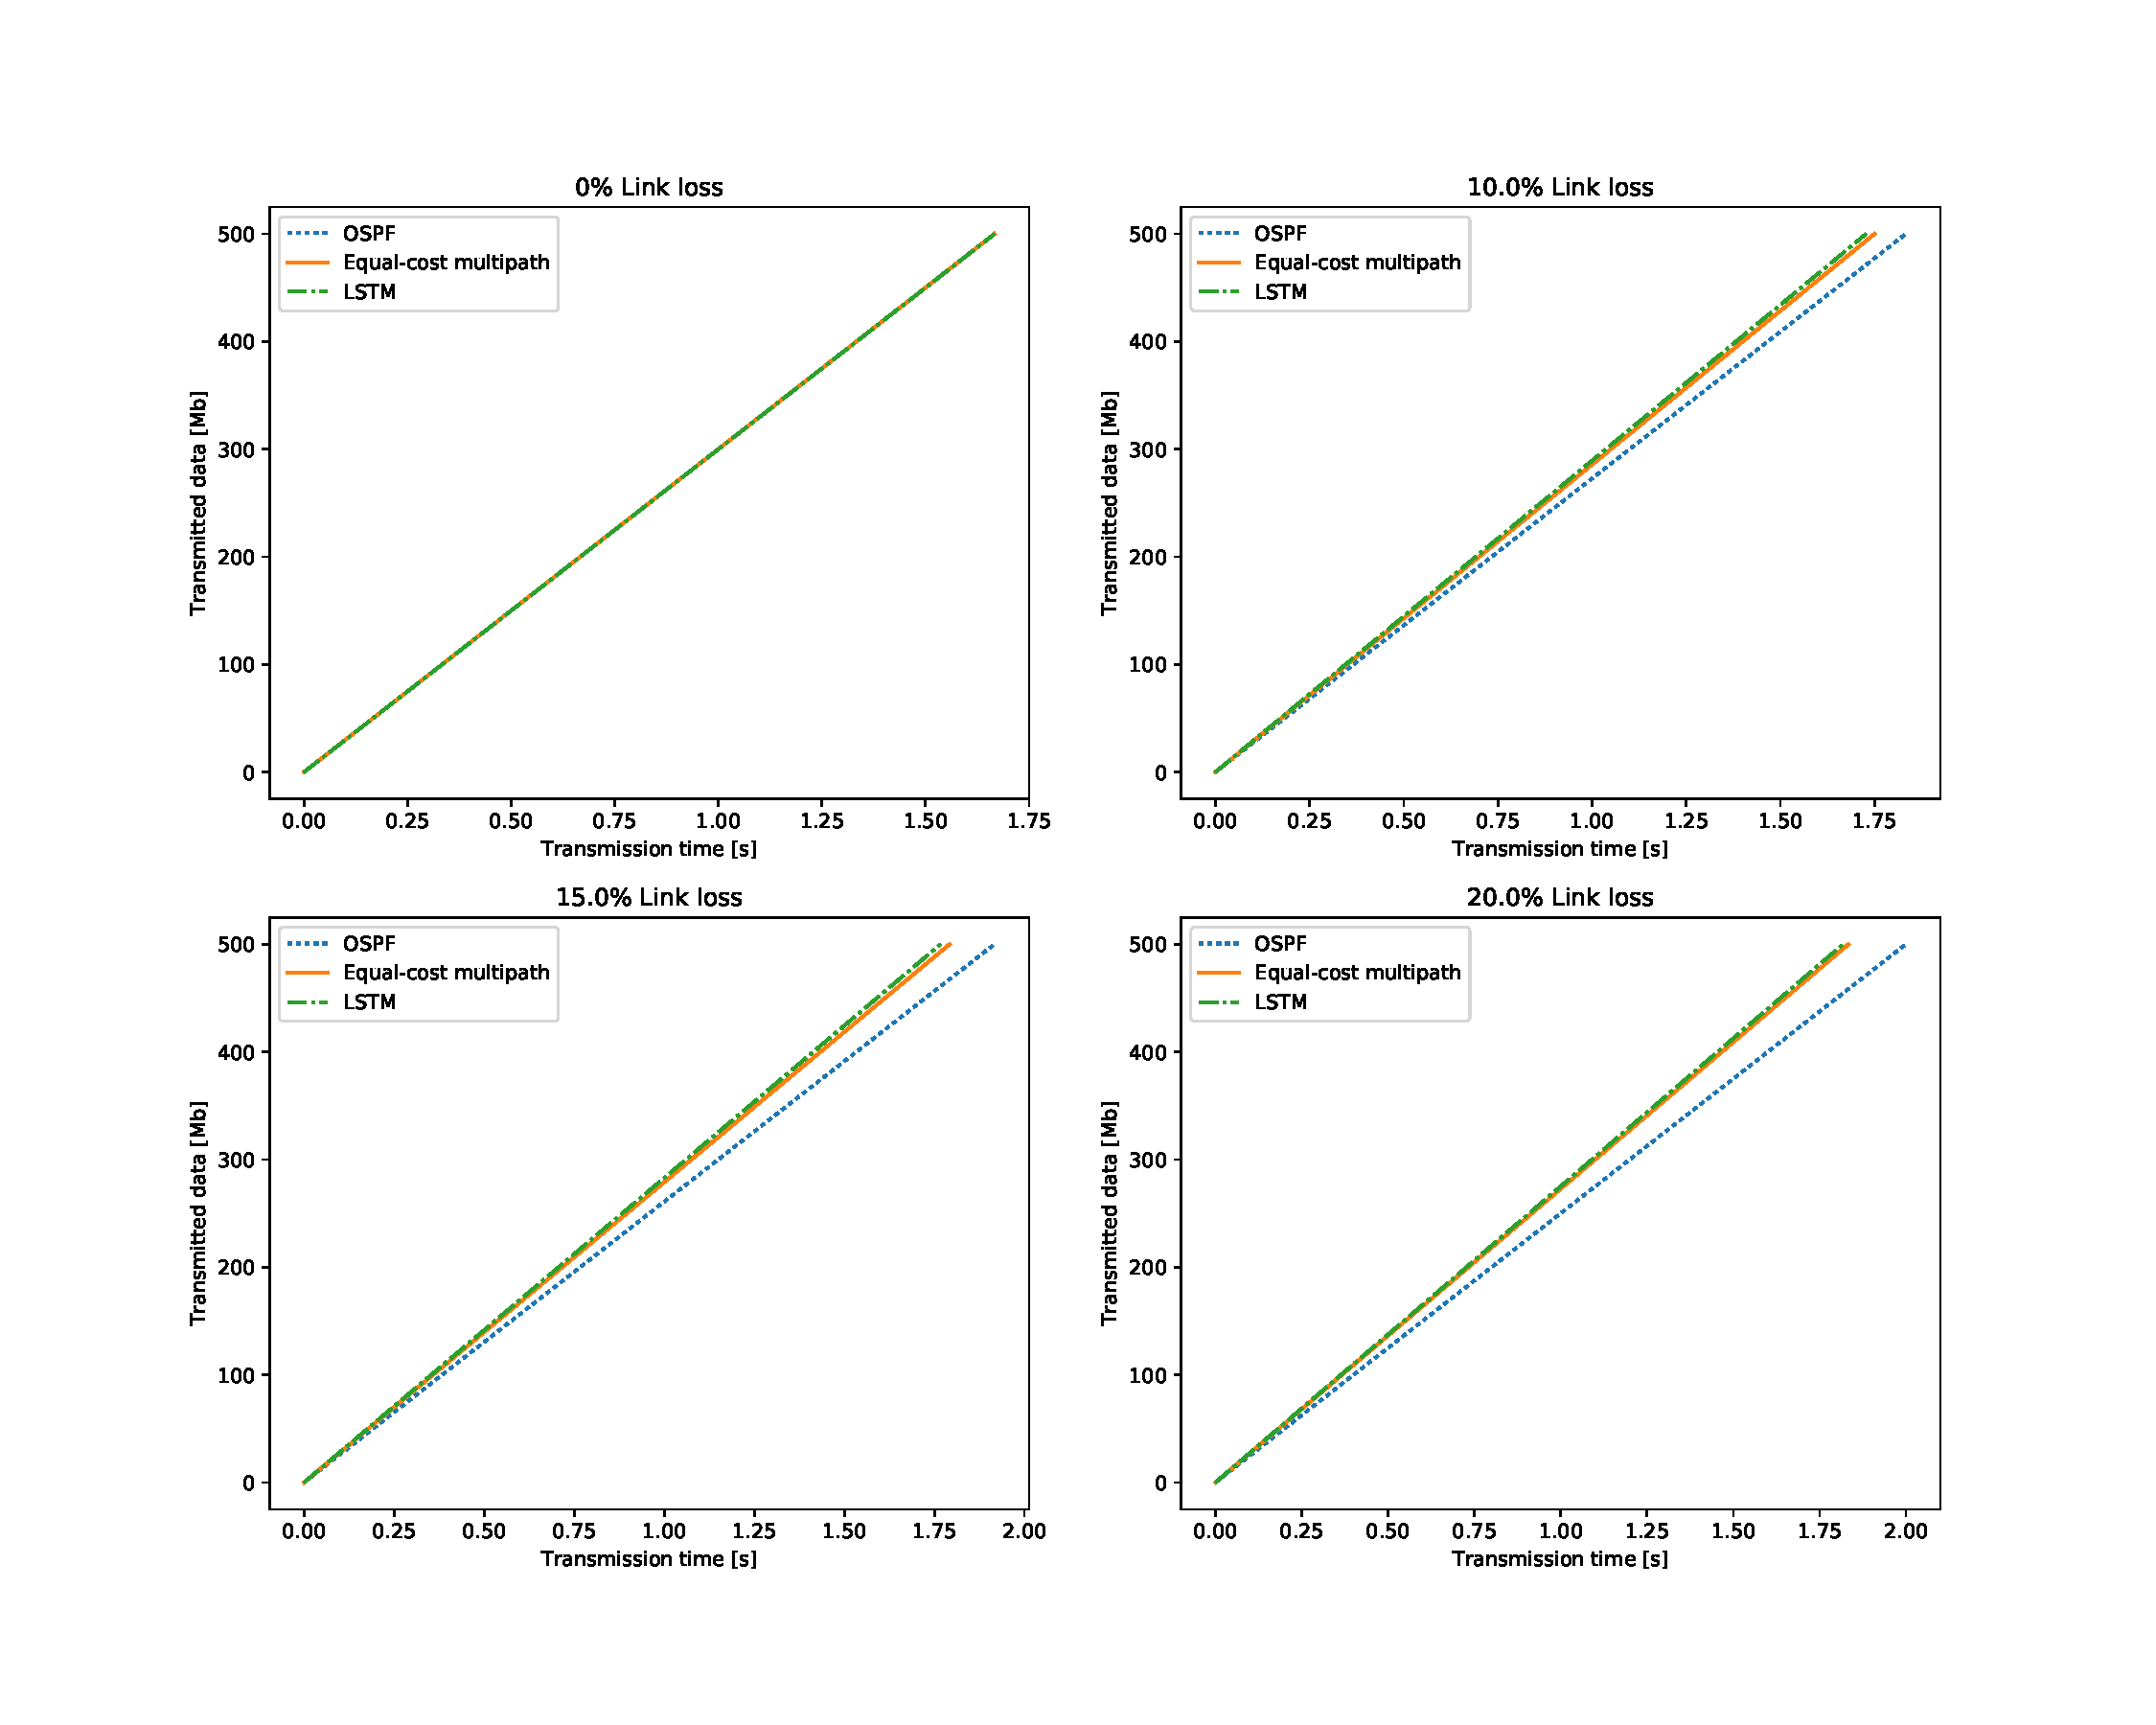
\includegraphics[width=0.88\paperwidth]{img/prediction_cmp}
}
\caption{Routing policies retransmission comparison.}
\label{fig:prediction_cmp}
\end{figure}